\chapter{Conclusioni}
Al termine dello sviluppo si è riusciti ad ottenere un classificatore di ADLs in grado di interagire con una applicazione Android.

\vspace{5mm} %5mm vertical space

Prendendo in considerazione le sole 3 attività scelte per la classificazione (camminata, corsa e salti) su cui abbiamo testato il riconoscimento 
e la partizione di cui abbiamo mostrato i risultati grafici durante la trattazione, siamo riusciti ad ottenere un buon riconoscimento 
delle attività con \textit{solamente} poco più di 250 mila record di dati.

\vspace{5mm} %5mm vertical space

L'aggiunta di ulteriori attività comporterebbe logicamente l'esigenza di incrementare le informazioni di apprendimento per mantenere 
invariata l'accuratezza del riconoscimento. Reputo entrambi questi passaggi fondamentali per l'utilizzo del 
classificatore nel mondo reale, oltre che per il riconoscimento di una quantità maggiore di ADLs.

\subsection*{Ottimizzazioni future}
Seppur già funzionante, l'intero sistema può essere ulteriormente migliorato. 
Sono stati ipotizzati dei possibili scenari per una futura ottimizzazione del sistema.

\subsubsection{Disponibilità offline}
Così come è stato presentato e realizzato il sistema dipende completamente dalla connessione di rete, nonché dalla comunicazione costante con il server 
durante una qualsiasi attività che preveda la raccolta dei dati.
Un'opportuna ottimizzazione sarebbe quella di rendere il tutto funzionante anche in assenza di connessione.

\vspace{5mm} %5mm vertical space
L'applicazione potrebbe raccogliere i dati inerziali di apprendimento all'interno di un database locale e procede all'invio al server 
anche in un secondo momento. La fase di riconoscimento potrebbe avvenire all'interno del dispositivo con l'utilizzo di Tensorflow Lite \cite{tensorflow_lite} 
e dei modelli pre-allenati scaricati dal server in un qualunque momento.

\vspace{5mm} %5mm vertical space
Con questa ottimizzazione il server avrà comunque una funzione chiave nell'intero sistema: l'aggregazione dei dati, la 
generazione dei modelli e la conversione degli stessi nel formato adatto.

\begin{figure}[H]
    \centering
    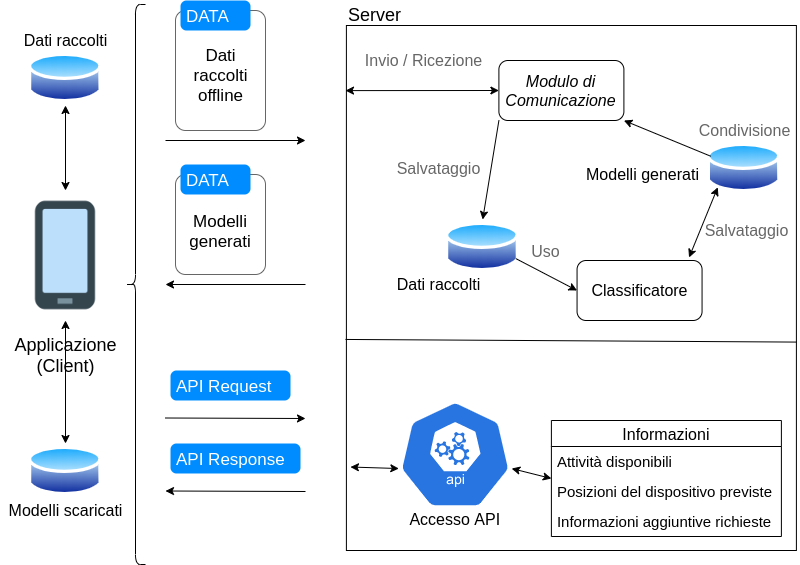
\includegraphics[scale = 0.56]{assets/images/future/offline.png}
    \caption{Ottimizzazione del progetto per l'utilizzo offline}
    \label{fig:overview}
\end{figure}

\subsubsection{Aggregazione dei sensori}
Al momento il riconoscimento delle attività si basa sull'utilizzo separato delle informazioni raccolte dai diversi sensori inerziali.
Uno dei partizionamenti visti sul set di dati completo è appunto quello riguardante il sensore utilizzato.

\vspace{5mm} %5mm vertical space

Quindi, oltre ai modelli \textit{"singoli"} che rimangono utili per l'eventualità in cui un particolare sensore non è presente oppure è disabilitato, 
potrebbe essere un'opportuna ottimizzazione l'inserimento di un nuovo modello in grado di considerare i dati ottenuti da entrambi 
i sensori.